% These abbreviations are used in figure labels and all figures are listed in the "List of Figures" some pages before.
% Reset them, so that they are expanded once in the text.
\glsreset{API}
\glsreset{PDB}
\glsreset{RPC}

\chapter{Basics}
This chapter introduces several Open-Source software projects relevant to the thesis implementation work.
It is followed by an explanation of the backgrounds and technical terms regarding Printing support in operating systems.
Finally, some utilities are presented, which have been widely used for the development of the Printing Stack.


\section{The ReactOS Project}
The ReactOS Project goes back to a project called \emph{FreeWin95} in 1996 by various software developers to create an Open-Source reimplementation of Microsoft Windows 95.
With no visible progress by the end of 1997, the project was restarted in 1998 as \emph{ReactOS} and shifted its goals towards providing an operating system compatible with the Microsoft Windows NT series under the GNU General Public License \cite{reactos1998news}.
The name was chosen to express the dissatisfaction with the Microsoft operating system monopoly and provide a \emph{reaction} to it \cite{sixtus2004reactos}.

Today, ReactOS strives for compatibility with Windows Server 2003 (also known as Windows NT 5.2) at the kernel level while applications can also make use of some functions found in more recent Windows releases \cite{guo2009newsletter54}.
Several popular Windows applications such as Adobe Photoshop or Microsoft Office are running natively under ReactOS.
This also applies to several drivers for hardware components such as graphics adapters, network cards, or sound cards.

By providing this level of compatibility with a very popular operating system, ReactOS aims to become a free and Open-Source alternative to it.
As a lightweight operating system, ReactOS can be a solution to keep older computers usable.
Finally, the Open-Source nature of ReactOS allows for customizations not possible with Microsoft Windows.
It also reduces licensing costs and ensures confidentiality in sensitive environments.


\section{The WINE Project}
The Open-Source WINE Project was founded in 1993 with the goal of running Windows applications under Linux.
In contrast to typical emulator software, WINE does not simulate a full x86 processor to run an operating system on it, but instead provides a loader for binaries in the Windows \gls{PE} format along with a set of reimplemented Windows libraries \cite{gardner1998winefaq}.
This allows applications to deliver a higher performance under WINE than under x86 emulators, but this performance benefit is getting lower with advancements in x86 virtualization technology.

In contrast to ReactOS, WINE does not provide any support for Windows device drivers.
The project also does not target a specific Windows version, but allows users to choose a particular Windows version WINE shall mimic.
Due to similar licenses, code of fundamental Windows libraries is frequently exchanged between the ReactOS and the WINE Project.


\section{Printing Support In Operating Systems}
Operating system support for Printing is as old as the Personal Computer itself, with support for then standard Dot-Matrix Parallel Port Printers being implemented into the original IBM Personal Computer 5150 \gls{BIOS} of 1981 \cite{brooks2015pcdos, powell2010lprng}.
As neither a concept of Printer Drivers nor a common Printer Control Language existed at that time, user programs were only able to output basic unformatted text by default.
Higher sophisticated printing of different fonts or graphics required software developers to implement support for each Printer Control Language into their applications.
This first changed with the introduction of the Apple LaserWriter Printer in 1985, which standardized Adobe PostScript as a vendor-independent Printer Control Language \cite{leurs2013postscript}.
Around the same time Windows 1.0 debuted, featuring a first Printing Stack consisting of a Print Spooler along with a set of Printer Drivers for converting \gls{GDI} output into different Printer Control Languages \cite{kolacki1987windows}.
Instead of talking directly to the Printer, applications now just needed to call \gls{GDI} functions for printing out a document. Usually, these are the same functions already used for displaying graphics and text on the screen.
The Spooler is responsible for enabling non-blocking access to a single shared Printer by multiple applications.

With Windows, Mac OS X, and Linux evolving into the three popular operating systems these days, two Printing Stacks remain.
These are described in the following sections.

\subsection{Microsoft Windows Printing Stack}
\label{sec:WindowsPrinting}
The Printing Stack of the Microsoft Windows Operating System is unique in the way that some higher level components maintain compatibility with all previous Windows versions. At the same time, lower level parts follow the latest principles of modern operating systems.
A schema of the Printing Process under Windows 2000 and later is given in Figures~\ref{fig:WindowsSpooling} and \ref{fig:WindowsPrinting}.
All components involved are explained in the following.
Yellow marked nodes denote components, for which compatible replacements are implemented within this thesis.

\begin{figure}[h]
	\centering
	
	\begin{tikzpicture}
		\node [cf_block, cf_impl] (App) {Application};
		\node [cf_block, below left = 20mm of App] (gdi32) {GDI\\gdi32.dll};
		\node [cf_block, cf_impl, below = 30mm of App] (winspool) {Spooler API\\winspool.drv};
		\node [cf_block, cf_impl, below = 20mm of winspool] (spoolsv) {Spooler Server\\spoolsv.exe};
		\node [cf_block, cf_impl, below = of spoolsv] (spoolss) {Spooler Router\\spoolss.dll};
		\node [cf_block, cf_impl, below left = 20mm and 32mm of spoolss] (localspl) {Local Spooler\\localspl.dll};
		\node [cf_block, below = 20mm of spoolss] (inetpp) {Internet Print Provider\\inetpp.dll};
		\node [cf_block, below right = 20mm and 40mm of spoolss] (win32spl) {LanMan Print Services\\win32spl.dll};
		\node [cf_block, right = 80mm of spoolsv] (extern_spoolsv) {Spooler Server\\on another computer};
		\node [cf_data, cf_impl, below = 20mm of localspl] (spoolfile) {Spool File};
		\node [cf_block, below = 20mm of inetpp] (ippprinter) {IPP-capable Printer};
		
		\path [cf_line, dotted] (App) -- (gdi32);
		\path [cf_line, dotted] (App) -- (winspool);
		\path [cf_line] (gdi32) -- (winspool);
		\path [cf_line] (winspool) -- (spoolsv);
		\path [cf_label] (winspool) edge node [right] {RPC Calls over\\ncalrpc protocol} (spoolsv);
		\path [cf_line] (spoolsv) -- (spoolss);
		\path [cf_line, dotted] (spoolss) -- (localspl);
		\path [cf_line, dotted] (spoolss) -- (inetpp);
		\path [cf_line, dotted] (spoolss) -- (win32spl);
		\path [cf_line] (localspl) -- (spoolfile);
		\path [cf_line] (inetpp) -- (ippprinter);
		
		\coordinate [left = 3mm of extern_spoolsv] (extern_spoolsv_anchor);
		\path [draw] (win32spl) -- (win32spl |- ippprinter.north);
		\path [draw] (win32spl |- ippprinter.north) -- (ippprinter.north -| extern_spoolsv_anchor);
		\path [draw] (ippprinter.north -| extern_spoolsv_anchor) -- (extern_spoolsv_anchor);
		\path [cf_label] (ippprinter.north -| extern_spoolsv_anchor) edge node [right] {RPC Calls over\\ncacn\_np protocol} (extern_spoolsv_anchor);
		\path [cf_line] (extern_spoolsv_anchor) -- (extern_spoolsv.west);
	\end{tikzpicture}
	
	\caption{Spooling a Print Job into a file as implemented in current Microsoft Windows Operating Systems}
	\label{fig:WindowsSpooling}
\end{figure}

User-Mode Windows applications interact with the operating system by calling documented \gls{API} functions from operating system \gls{DLL} files.
To print out a document, an application usually begins by composing the document out of graphics and text using \gls{GDI} functions (implemented in \emph{gdi32.dll}).
Afterwards, \gls{GDI} serializes the drawing commands into the \gls{EMF} format and uses Spooler \gls{API} functions to set up a new Print Job.
The generated \gls{EMF} data is then passed to the Print Job.
If the application does not need to compose the document, but already has prepared data in a format supported by the Print Processor, it can skip the route through \gls{GDI} and call the Spooler \gls{API} functions directly \cite{yuan2001windows}.

For historical reasons, the Spooler \gls{API} is implemented in a file called \emph{winspool.drv}.
Despite its different extension, this file has the same structure as other operating system \gls{DLL} files.
An individual instance of \emph{winspool.drv} is loaded with every application that uses functions of the Windows Printing Stack.
Its \gls{API} can be categorized as follows:

\begin{itemize}
	\item Opening handles to Ports, Print Monitors, Print Servers, and Printers (all through \texttt{OpenPrinter} \cite{msdn2015openprinter})
	\item Performing further operations on these opened objects (e.g. preparing a new document with \texttt{StartDocPrinter} or retrieving information with \texttt{GetPrinter})
	\item Adding, deleting, and enumerating available Forms, Ports, Print Monitors, Print Processors, Printers, Printer Configuration Data, Printer Connections, and Printer Drivers as well as their properties (\texttt{Add*}, \texttt{Delete*}, and \texttt{Enum*} group of functions)
	\item Receiving notifications about status changes inside the Printing Stack \\ (\texttt{*PrinterChangeNotification} group of functions)
	\item Providing User Interfaces to let the user configure Printer and Print Job settings
\end{itemize}

As every application loads its own instance of \emph{winspool.drv}, the operating system needs to provide a single service, which is loaded only once and centrally manages Printer utilization.
This instance is the Spooler Server, which is implemented as a Windows Service in the module \emph{spoolsv.exe}.
Communication between \emph{winspool.drv} and \emph{spoolsv.exe} happens through \glspl{RPC}.
\gls{RPC} is a popular concept for enabling a process to call a function in another process, even on another computer, without writing any network-specific code.
Almost every \emph{winspool.drv} function performs an \gls{RPC} call to the matching counterpart function in the Spooler Server.
\gls{RPC} calls are further discussed in Section~\ref{sec:rpc}.

Accepting \gls{RPC} calls of all users requires the Spooler Server to be a high-privileged process.
This bears some security risks as a possibly vulnerable \gls{RPC} call could be used to let a low-privileged client run code in the security context of the high-privileged Spooler Server.
To mitigate this possible attack, the Spooler Server employs the concept of \emph{Impersonation}.
The Impersonation feature of Windows allows a thread to temporarily drop its high privileges by switching to the security context of another user \cite{technet2015impersonation}.

In the case of the Spooler Server, every \gls{RPC} call is implemented as follows:
First of all, the Spooler Server impersonates the calling client.
Afterwards, a matching function in the Spooler Router is called (implemented in \emph{spoolss.dll}).
The Spooler Router offers such a counterpart to each \gls{RPC} call.
Finally, the security context of the Spooler Server is restored and the \gls{RPC} call returns.
This ensures a clean separation between code running in the high-privileged Spooler Server security context and code running in the low-privileged user context.
The entire process is exemplified for a \texttt{WritePrinter} call in Figure~\ref{fig:WritePrinterProcessing}.
The full listing for the implemented ReactOS \gls{RPC} server function can be found in Appendix~\ref{sec:RpcWritePrinter}.

\begin{figure}[h]
	\centering
	
	\begin{tikzpicture}
		\node [cf_head, minimum width = 68mm] (UserContext) {Low-privileged User Context};
		\node [cf_head, minimum width = 68mm, right = 73mm of UserContext] (SystemContext) {High-privileged System Context};
	
		\node [cf_block, below = of UserContext] (App) {Application calls \texttt{WritePrinter}\\in \emph{winspool.drv}};
		\node [cf_block, below = 22mm of App] (RpcWritePrinter) {\emph{winspool.drv} calls \texttt{\_RpcWritePrinter}\\to perform an RPC call to\\the Spooler Server};
		\node [cf_block, below = 60mm of SystemContext] (RpcImpersonateClient) {Spooler Server calls\\\texttt{RpcImpersonateClient}\\to impersonate the caller};
		\node [cf_block, below = 43mm of RpcWritePrinter] (WritePrinter) {Spooler Server calls matching\\\texttt{WritePrinter} in Spooler Router};
		\node [below = 5mm of WritePrinter] (Additional) {...};
		\node [cf_block, below = 12mm of Additional] (RpcRevertToSelf) {Spooler Server calls \texttt{RpcRevertToSelf}\\to switch back to its own security context};
		\node [cf_block, below = 63mm of RpcImpersonateClient] (Return) {Spooler Server returns the\\error code of its performed\\\texttt{WritePrinter} call};
		
		\path [cf_line] (App) -- (RpcWritePrinter);
		
		\coordinate [below = 3mm of RpcWritePrinter] (RpcWritePrinter_anchor);
		\path [draw] (RpcWritePrinter) -- (RpcWritePrinter_anchor);
		\path [draw] (RpcWritePrinter_anchor) -- (RpcWritePrinter_anchor -| RpcImpersonateClient);
		\path [cf_line] (RpcWritePrinter_anchor -| RpcImpersonateClient) -- (RpcImpersonateClient);
		
		\coordinate [below = 3mm of RpcImpersonateClient] (RpcImpersonateClient_anchor);
		\path [draw] (RpcImpersonateClient) -- (RpcImpersonateClient_anchor);
		\path [draw] (RpcImpersonateClient_anchor) -- (RpcImpersonateClient_anchor -| WritePrinter);
		\path [cf_line] (RpcImpersonateClient_anchor -| WritePrinter) -- (WritePrinter);
		
		\path [draw] (WritePrinter) -- (Additional);
		\path [cf_line] (Additional) -- (RpcRevertToSelf);
		
		\coordinate [below = 3mm of RpcRevertToSelf] (RpcRevertToSelf_anchor);
		\path [draw] (RpcRevertToSelf) -- (RpcRevertToSelf_anchor);
		\path [draw] (RpcRevertToSelf_anchor) -- (RpcRevertToSelf_anchor -| Return);
		\path [cf_line] (RpcRevertToSelf_anchor -| Return) -- (Return);
		
		\coordinate [below = 2mm of Return] (Return_anchor);
		
		\begin{pgfonlayer}{background}
			\fill [fill=green!20] (UserContext.north west) rectangle (UserContext.east |- Return_anchor);
			\fill [fill=red!20] (SystemContext.north west) rectangle (SystemContext.east |- Return_anchor);
		\end{pgfonlayer}
	\end{tikzpicture}
	
	\caption{Using Impersonation to switch between security contexts while processing an \texttt{WritePrinter} call}
	\label{fig:WritePrinterProcessing}
\end{figure}

The Spooler Router derives the name from its principal task, namely routing an incoming function call to one or more Print Providers.
These Print Providers also offer a counterpart to each function implemented in the Spooler Router.
Due to the nature of the functions, there are basically three ways how a Spooler Router function is implemented:

\begin{itemize}
	\item Subsequently route a function call to every available Print Provider until one of them indicates success.
	      This is done for e.g. the \texttt{OpenPrinter} function to determine the Print Provider that can handle the respective Printer.
	\item Directly route the function call to the Print Provider, for which a previous \texttt{OpenPrinter} call succeeded.
	      This is done for all functions accepting a handle returned by \texttt{OpenPrinter}.
	\item Route the function call to all available Print Providers and collect the returned information.
	      This is done for e.g. \texttt{EnumPrinters} to retrieve information about all available Printers.
\end{itemize}

Windows ships with these Print Providers by default:

\begin{itemize}
	\item The Local Spooler (implemented in \emph{localspl.dll}) handles Printers locally connected to the computer.
	\item The Internet Print Provider (implemented in \emph{inetpp.dll}) forwards calls to Remote Printers using the \gls{IPP}.
	\item The LanMan Print Services (implemented in \emph{win32spl.dll}) are used when accessing Remote Printers shared by another Windows computer.
\end{itemize}

Another Print Provider (\emph{nwprovau.dll}) for accessing Printers on Novell NetWare servers used to be available, but became largely irrelevant due to the demise of the NetWare Operating System.
It has finally been removed in Windows Vista.
The extensible architecture enables third-party vendors to ship additional Print Providers for supporting other protocols.

In the following, we only take a look at the Local Spooler.
The Local Spooler finally does the real work of managing the Print Queues for all locally connected Printers instead of passing on the received function call to another module.
Synchronous communication between computers and Printers can be a major bottleneck.
Therefore, the Local Spooler first writes the received data to print into a so called Spool File and then starts a thread to transmit that Spool File to the Printer.
This enables the users to continue their work in the application while the Local Spooler transmits the Spool File to the Printer in the background.
Without this two-stage process, the application would be blocked until the last page of the entire Print Job has finished printing.

\begin{figure}[h]
	\centering
	
	\begin{tikzpicture}
		\node [cf_data, cf_impl] (spoolfile) {Spool File};
		\node [cf_block, cf_impl, right = 30mm of spoolfile] (winprint) {Print Processor\\winprint.dll};
		\node [cf_block, right = 50mm of winprint] (printerdll) {Printer Driver\\Graphics DLL};
		\node [cf_block, below right = 18mm of printerdll] (gdi32) {GDI\\gdi32.dll};
		\node [cf_block, cf_impl, below = 20mm of winprint] (spoolss) {Spooler Router\\spoolss.dll};
		\node [cf_block, cf_impl, below = of spoolss] (localspl) {Local Spooler\\localspl.dll};
		\node [cf_block, below = 20mm of localspl] (pjlmon) {Language Monitor\\pjlmon.dll};
		\node [cf_block, cf_impl, below left = 28mm of pjlmon] (localmon) {Local Port Monitor\\localmon.dll};
		\node [cf_block, below right = 28mm of pjlmon] (usbmon) {USB Port Monitor\\usbmon.dll};
		\node [cf_block, below = 35mm of pjlmon] (kernel32) {User-Mode Kernel API for accessing a port\\kernel32.dll};
		\node [cf_block, below = of kernel32] (printer) {Printer};
		
		\path [cf_line] (spoolfile.east) -- (winprint.west);
		\path [cf_line, dotted] (winprint.east) -- (printerdll);
		\path [cf_label] (winprint.east) edge node [above] {For EMF datatype} (printerdll);
		\path [cf_line] (printerdll) -- (gdi32);
		\path [cf_line] (gdi32.100) -- (printerdll.-30);
		\path [draw] (printerdll) -- (printerdll |- spoolss);
		\path [cf_line] (printerdll |- spoolss) -- (spoolss);
		\path [cf_label] (printerdll |- spoolss) edge node [above] {Converted to RAW datatype} (spoolss);
		\path [cf_line, dotted] (winprint) -- (spoolss);
		\path [cf_label] (winprint) edge node [right] {For RAW datatype} (spoolss);
		\path [cf_line] (spoolss) -- (localspl);
		\path [cf_line, dotted] (localspl) -- (pjlmon);
		
		\coordinate [below = 3mm of pjlmon] (pjlmon_anchor_half);
		\coordinate [below = 6mm of pjlmon] (pjlmon_anchor);
		\path [cf_line] (pjlmon) -- (pjlmon_anchor);
		\path [cf_line, dotted] (pjlmon_anchor) -- (localmon);
		\path [cf_line, dotted] (pjlmon_anchor) -- (usbmon);
	
		\coordinate [below right = 9mm of localspl] (localspl_anchor);
		\path [draw, dotted] (localspl.-40) -- (localspl.-40 |- localspl_anchor);
		\path [draw, dotted] (localspl.-40 |- localspl_anchor) -- (localspl_anchor);
		\path [draw, dotted] (localspl_anchor) -- (localspl_anchor |- pjlmon_anchor_half);
		\path [cf_line, dotted] (localspl_anchor |- pjlmon_anchor_half) -- (pjlmon_anchor_half);
		
		\path [cf_line] (localmon) -- (kernel32.north -| localmon);
		\path [cf_line] (usbmon) -- (kernel32.north -| usbmon);
		\path [cf_line] (kernel32) -- (printer);
	\end{tikzpicture}
	
	\caption{Printing from a Spool File as implemented in current Microsoft Windows Operating Systems}
	\label{fig:WindowsPrinting}
\end{figure}

The started thread now loads the Print Processor (implemented in \emph{winprint.dll} since Windows Vista, previously part of \emph{localspl.dll}), which is responsible for reading the print data from the Spool File and applying Print Job specific settings.
These include settings like Multiple Copies, Collation, Reverse Printing, Duplex Printing or N-up Printing.
Available options in this regard highly depend on the datatype of the print data.
A Printer vendor can provide its own Print Processor to support additional options instead of using the Windows default one.

If the datatype is RAW, the print data is assumed to be of a Printer Control Language and the Print Processor simply passes it on without any further processing.
For the \gls{EMF} datatype, Print Job specific settings are applied first before the print data is converted into Printer Control Language.
The conversion is performed using a Printer Graphics \gls{DLL} supplied by the Printer vendor, which heavily uses functions from \gls{GDI} to convert the \gls{EMF} data.
The Printer Graphics \gls{DLL} is also called the actual Printer Driver, because it is the only component specific to the Printer in this process.

In a next step, Spooler Router functions are used to transmit the print data in a Printer Control Language to a Print Monitor.
Two types of Print Monitors exist: Language Monitors and Port Monitors.
A Language Monitor is written for a specific Printer Job Language to communicate bidirectionally with the Printer.
This communication enables the Monitor to receive detailed Printer status information or add control codes to the print data before passing it to the Port Monitor.
Control codes can be used to set a wide range of options.
One example is switching between multiple Printer Control Languages supported by the Printer.

If the Printer does not require such control codes, the Language Monitor can be skipped and the print data directly flows to the Port Monitor.
By default, Windows ships with a Language Monitor that implements the HP PJL Printer Job Language \cite{msdn2015langmonitors}.

A Port Monitor is responsible for managing unidirectional data output to a physical computer port.
Depending on the type of port, this can range from simply opening the port through a kernel function (like Parallel Ports) to performing a complex wireless detection sequence (for Infrared Printers).
The following Port Monitors are shipped with Windows:

\begin{itemize}
	\item The Local Port Monitor (implemented in \emph{localmon.dll} until Windows NT 4.0, part of \emph{localspl.dll} since Windows 2000) manages Parallel, Serial, and Infrared Ports as well as redirecting the printing output into a file.
	\item The USB Port Monitor (implemented in \emph{usbmon.sys}) manages Printers connected to a \gls{USB} port.
\end{itemize}

This architecture again provides support for additional Print Monitors.
Such extensibility is heavily used by third-party companies.
For example, Adobe has implemented a \gls{PDF} Port Monitor for a virtual \gls{PDF} Printer that converts the print data into a \gls{PDF} file \cite{adobe2015printerproperties}.


\subsection{Common UNIX Printing System (CUPS)}
The \gls{CUPS} was developed and released by Michael Sweet in 1999 to address the lack of a standard printing interface in UNIX-based operating systems (such as Linux) at that time \cite{sweet1999cups}.
Previously, there were two competing systems, namely the System V Printing System (lp) and the Berkeley Printing System (lpr), which were incompatible to each other and only supported text and PostScript printing.
Printing other formats required third-party tools to account for the vast majority of available Printers.

\gls{CUPS} has quickly emerged as the de-facto standard Printing Stack under Linux, with User Interfaces being available for the two major desktops KDE and GNOME \cite{pfeifle2001kdeprint} \cite{burton2003gnome}.
\gls{CUPS} has also been adopted by Apple in 2002 to serve as the Printing System for Mac OS X 10.2 and later versions \cite{esp2002applecups}.

The architecture of \gls{CUPS} is depicted in Figure~\ref{fig:CUPSArchitecture}.

\begin{figure}[h]
	\centering
	
	\begin{tikzpicture}
		\node [cf_block] (app) {Application};
		\node [cf_block, below left = 15mm and 20mm of app] (cups-lpd) {cups-lpd Daemon};
		\node [cf_block, below = 30mm of app] (cupsapi) {CUPS\\API};
		\node [cf_block, below = of cupsapi] (cupsd) {CUPS Daemon};
		\node [cf_block, below = of cupsd] (prefilter) {Prefilter};
		\node [cf_block, below left = 15mm of prefilter] (pstops) {pstops};
		\node [cf_block, below left = 20mm and 12mm of pstops] (foomatic-rip) {foomatic-rip};
		\node [cf_block, below right = 12mm and 18mm of pstops] (pstoraster) {pstoraster};
		\node [cf_block, below = of pstoraster] (printerfilter) {Printer-specific\\filter};
		\node [cf_block, below = 50mm of prefilter] (backend) {CUPS Backend};
		\node [cf_block, below = of backend] (printer) {Printer};
		
		\path [cf_line, dotted] (app) -- (cups-lpd);
		\path [cf_label] (app) edge node [left] {LPD protocol} (cups-lpd);
		\path [cf_line, dotted] (app.-20) -- (app.-20 |- cupsd.north);
		\path [cf_label] (app.-20) edge node [right] {IPP protocol} (app.-20 |- cupsd.north);
		\path [cf_line, dotted] (app) -- (cupsapi);
		\path [cf_line] (cups-lpd) -- (cupsapi);
		\path [cf_line] (cupsapi) -- (cupsd);
		\path [cf_label] (cupsapi) edge node [left] {IPP protocol} (cupsd);
		\path [cf_line, dotted] (cupsd) -- (prefilter);
		\path [cf_line, dotted] (pstops |- cupsd.south) -- (pstops);
		\path [cf_line, dotted] (prefilter) -- (pstops);
		\path [cf_line, dotted] (pstops) -- (foomatic-rip);
		\path [cf_line, dotted] (pstops.-50) -- (backend.north -| pstops.-50);
		\path [cf_line, dotted] (pstops) -- (pstoraster);
		\path [cf_line] (foomatic-rip) -- (backend.165);
		\path [cf_line] (pstoraster) -- (printerfilter);
		\path [cf_line] (printerfilter) -- (backend);
		\path [cf_line] (backend) -- (printer);
	\end{tikzpicture}
	
	\caption{Architecture of the Common UNIX Printing System}
	\label{fig:CUPSArchitecture}
\end{figure}

An application can initiate a Print Job with \gls{CUPS} in three different ways.
The most common one is using the \texttt{cupsPrintFile} function (or a similar one) of the \gls{CUPS} C \gls{API} to print a file of a known filetype.
The \gls{API} function then initiates a Request over the \gls{IPP} protocol to a \gls{CUPS} instance on a local or remote computer.
As \gls{IPP} is a documented plaintext protocol based on \gls{HTTP}, an application can also easily generate a similar \gls{IPP} request itself and transmit it to the \gls{CUPS} Daemon without using the \gls{CUPS} \gls{API}.
Finally, \gls{CUPS} also provides the \emph{cups-lpd} daemon to provide compatibility with older applications using the \gls{LPD} protocol of the Berkeley Printing System.
cups-lpd translates incoming \gls{LPD} Requests to the \gls{IPP} protocol using the \gls{CUPS} \gls{API}.

In all three cases, the Print Request arrives at the \gls{CUPS} Daemon.
Depending on the Print Job settings and Printer utilization, the Job is processed immediately or scheduled for later.
When processing the Job, \gls{CUPS} first checks its filetype.
PostScript files can instantly be forwarded to the \emph{pstops} program while other filetypes need a conversion to PostScript format by the so called \emph{prefilter} first.
\gls{CUPS} can support any filetype, for which a converter program to PostScript exists, like plaintext files, image formats or web pages.
Filetypes and converter programs are determined using the system-wide \gls{MIME} database available on every UNIX-based operating system.
In a next step, the converter program is called and its output is fed to the \emph{pstops} program.

The \emph{pstops} program expects a PostScript input file and applies Print Job specific settings like N-up Printing or extracting a page range to print.
It also normalizes the input to account for the paper format of the target Printer.

The type of Printer used decides about the next step.
If the target Printer understands PostScript, the output from \emph{pstops} can directly be submitted to a \gls{CUPS} Backend.
Otherwise, the next step depends on whether \gls{CUPS} natively provides support for the target Printer.
If it does, the output is first converted to a \gls{CUPS} raster image file format using the \emph{pstoraster} tool and then sent to a Printer-specific filter, which generates data in a Printer Control Language from it.
Finally, that data is submitted to a \gls{CUPS} Backend as well.
If \gls{CUPS} does not natively support the target Printer, a solution may still be found in the third-party Foomatic Project.
The Foomatic Project provides a set of programs that convert PostScript data to various Printer Control Languages without utilizing an intermediate raster format.
If the Printer is supported by the Foomatic Project, \emph{pstops} passes its output to the \emph{foomatic-rip} program, which in turn outputs data in a Printer Control Language and submits it to a \gls{CUPS} Backend \cite{pfeifle2002cups}.

\gls{CUPS} provides several backends for transferring the received data to the actual Printer.
The type of backend used depends on the port and location of the target Printer.
For example, this can be a Printer connected to a Parallel, Serial, or USB port as well as a Remote Network Printer communicating over e.g. \gls{IPP}, \gls{SMB} or JetDirect protocol.


\subsection{Comparison Of Both Systems}
A neutral comparison of both Printing Stacks is not possible, because they were designed in different epochs, on different operating system architectures, and with different compatibility targets and different third-party support strategies in mind.
However, some major differences between both systems are outlined in this section.

The Windows Printing Stack allows third-party Printer vendors to add support for their Printer by implementing a custom Printer Graphics \gls{DLL}.
This \gls{DLL} file is then responsible for converting data from \gls{EMF} format to a Printer Control Language.
On the other hand, \gls{CUPS} provides several ways to add support for a new Printer.
The program for converting data to Printer Control Language could be a filter program that takes the \gls{CUPS} raster data as input.
It could also be a Foomatic plugin that directly operates on PostScript input data.
This offers developers more flexibility, but shifts the complexity to the user, who has to know what type of \gls{CUPS} Printer support the Printer vendor implemented.
Based on this information, different steps need to be taken to install the Printer.

\gls{CUPS} follows the UNIX principle of one program per task, so it divides its processing into several individual programs.
From one processing step to another, process parameters are constructed, a new process is created and its parameters are parsed.
Afterwards, the print data output of the previous process is copied to the new process by writing it to its standard input handle.
The whole procedure requires process creation on the underlying operating system to be a relatively cheap operation in order to make the performance loss involved negligible.
Some overhead is also added due to the construction and parsing of process parameters.
On the other hand, the Windows Printing Stack interfaces between different components by using C function calls and passing memory pointers.
This works with no additional overhead and does not add implications to the performance of the underlying operating system.

One may also expect severe scalability differences when comparing both Printing Stacks at serving Print Requests for a high number of clients.
Traditionally, the Print Server needs to perform the expensive task of converting the incoming print data to Printer Control Language for all clients.
When a \gls{CUPS} instance is configured on both the client and server though, the \gls{CUPS} architecture provides a way to offload data conversion to the clients and only send converted data in a Printer Control Language to the target Print Server.
Starting with Windows Vista, Microsoft has also introduced this feature in the Windows Printing Stack under the name \emph{Client-Side Rendering} \cite{msdn2015csr}.
Therefore, both Printing Stacks perform equally well at serving a high number of clients nowadays.


\section{Remote Procedure Call}
\label{sec:rpc}
\glsreset{RPC}
A \gls{RPC} is an interprocess communication concept to let programs execute functions in other programs, which are typically running on a different computer.
The required information about the function call and its parameters are transmitted over the network.
\gls{RPC} is widely adopted due to the fact that it abstracts these network communication details away from the developer.
This way, a remote function call be done just as easy as a local one and the developer does not need to write network-specific code.

The first popular implementation was the Open Network Computing Remote Procedure Call for UNIX-based operating systems proposed by Sun Microsystems in 1984 \cite{callaway2010sunrpc} (also called \emph{Sun RPC}).
Nowadays, popular implementations include Java's object-oriented \gls{RMI} as well as Microsoft's implementation called \emph{MSRPC} integrated into Windows.
Latter one is further illustrated in this section.

MSRPC is derived from the Open Software Foundation's Distributed Computing Environment DCE/\gls{RPC} implementation and first appeared in Windows NT 3.1 \cite{black1993msrpc}.
Among other details, it extends the DCE implementation with additional parameter types and transport protocols while still maintaining backwards compatibility with it \cite{microsoft2015msrpce}.

To make use of MSRPC, a developer has to define an interface through a supplemental file written in \gls{IDL}.
This file contains prototypes for all functions to be called remotely, annotated with details about their input and output parameters as well as the length of the data transferred through each parameter.
Afterwards, Microsoft's MIDL compiler is used to generate C code out of an \gls{IDL} file, separately for the client and server applications.
The developer can then write both applications communicating with each other.
Finally, each application is linked against Windows' \emph{rpcrt4.dll} library, which is responsible for the underlying network communication happening in the background.

Every function defined in the \gls{IDL} file can be called in the client application and the call arrives at a function with the same name defined in the server application.
This happens in the following way:

\begin{enumerate}
	\item The client calls a function defined in the interface.
				This actually calls the generated client code by the MIDL compiler.
	\item The generated code composes a network message out of the function name and all given parameters.
				This process is called \emph{Marshalling}.
	\item The network message is sent by the client and received by the server application.
	\item The generated code of the server application reconstructs the function name and its parameters out of the message.
				This process is called \emph{Unmarshalling}.
	\item With all this information, the generated code calls the respective implemented function in the server application.
\end{enumerate}

MSRPC builds the basis for several Windows core components, one of them being the Print Spooler.
As illustrated in Figure~\ref{fig:WindowsSpooling}, \gls{RPC} communication happens locally between the Spooler \gls{API} in \emph{winspool.drv} and the Spooler Server in \emph{spoolsv.exe}.
It also happens remotely from the LanMan Print Services component in \emph{win32spl.dll} to a Spooler Server on a different computer.
Two different \gls{RPC} protocols are used here, which are explained in the following:

\begin{itemize}
	\item \textbf{ncalrpc} \\
				The Network Computing Architecture Local Remote Procedure Call Protocol represents the most efficient way to perform an \gls{RPC} call, when client and server application both reside on the same computer \cite{msdn2015protseq}.
				This is the case for \emph{winspool.drv} and \emph{spoolsv.exe}.
	\item \textbf{ncacn\_np} \\
				The Network Computing Architecture Connection-Oriented Named Pipe Protocol supports an \gls{RPC} call between different computers relying on Named Pipes for the network transport \cite{microsoft2015msrpce}.
				Named Pipes represent a high-performance communication method integrated into Windows.
				This protocol is well suited for communication between \emph{win32spl.dll} and a remote \emph{spoolsv.exe} instance.
\end{itemize}

A deeper look into \gls{RPC} would go beyond the scope of this thesis.
Refer to \cite{shirleyrosenberry1995msrpc} for further information on this topic.


\section{Reverse Engineering Tools}
Reverse Engineering in Computer Science or \gls{RCE} is the process of examining an existing software or technology in order to gather enough details for an own reimplementation that is compatible to the original.
Various legal methods backed by court decisions exist to perform this process without infringing copyrights.
These are commonly referred to as \emph{Clean-room Reverse Engineering}.

Popular realizations of Reverse Engineering include the creation of a 100\% compatible reimplementation of the IBM PC \gls{BIOS} by Compaq Computer Corporation for its own computers in 1982.
This step was fundamental to the computer industry as it paved the way for a large upcoming market of IBM-compatible computers.
Reverse Engineering techniques have also been used during the development of the LibreOffice Productivity Suite to enable compatibility with Microsoft Office file formats. The LibreOffice implementation is available for more operating systems, increases competition on this market and avoids a vendor lock-in to products of a single company.

With Microsoft Windows being the most popular closed-source operating system, several advanced tools for Clean-room Reverse Engineering under Windows exist.
Some of them have been used during the thesis work and are presented in the following.


\subsection{Dependency Walker}
\glsreset{DLL}
The Dependency Walker tool provides an overview of the \glspl{DLL} referenced by a module as well as the exported and imported \gls{API} functions from this module.
It thereby offers a good entry point into figuring out the purpose of a module and its dependencies with other modules.
The tool is bundled with a number of Microsoft development products and also available as a free download from \href{http://www.dependencywalker.com}{www.dependencywalker.com}. 
A screenshot of the Dependency Walker user interface is given in Figure~\ref{fig:DependencyWalker}.
It clearly shows the exported \gls{API} functions \texttt{GetPrintProcessorCapabilities}, \texttt{InitializePrintMonitor}, and \texttt{InitializePrintProvidor} of Windows Server 2003's \emph{localspl.dll}.
From this fact, one can conclude that this \emph{localspl.dll} integrates the three distinct components Print Monitor, Print Processor, and Print Provider into a single module.

\begin{figure}[t]
	\centering
	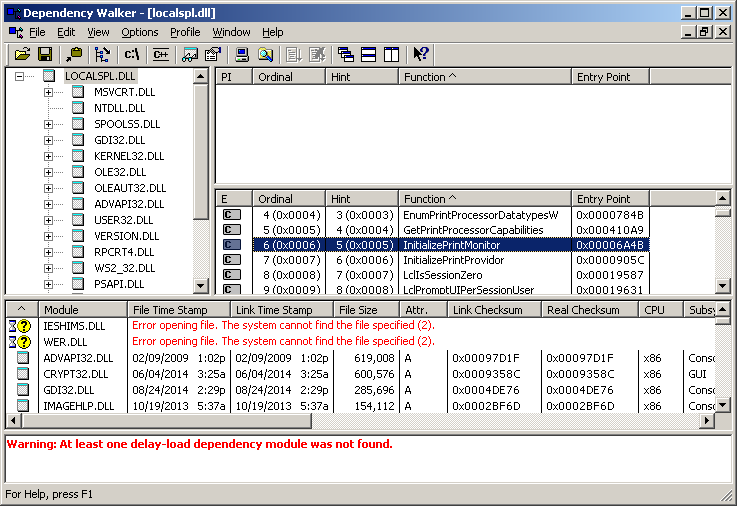
\includegraphics{images/depends.png}
	\caption{The Dependency Walker tool used to analyze the \emph{localspl.dll} of Windows Server 2003}
	\label{fig:DependencyWalker}
\end{figure}


\subsection{GNU strings}
The GNU strings utility reads any binary file and outputs all found sequences of printable characters.
It supports interpretation of the characters as ANSI and Unicode strings, which is a requirement for analyzing Windows applications that often use both character sets.
The tool reveals many interesting strings contained in Windows modules, for example:

\begin{itemize}
	\item Registry keys used to store the module's settings
	\item Paths to other related files
	\item Template data used by the module to fulfill its tasks
	\item Error messages (useful to get an idea what tasks are fulfilled by the module)
\end{itemize}

GNU strings is part of the Open-Source GNU Binutils package and shipped with many Linux distributions \cite{fsf2015strings}.
A Windows version of the tool is part of the \href{https://www.reactos.org/wiki/Build_Environment}{ReactOS Build Environment}.


\subsection{Rohitab Batra's API Monitor}
The \gls{API} Monitor by Rohitab Batra is a freely downloadable tool from \href{http://rohitab.com}{rohitab.com}.
It offers an efficient graphical user interface for monitoring the \gls{API} function calls of selected applications.
For \gls{API} functions known to the tool, the supplied parameter values are extracted and passed structures are decomposed.
The application can be enhanced to monitor additional \gls{API} functions by writing simple function definition files in \gls{XML}.
A screenshot of the tool is given in Figure~\ref{fig:APIMonitor}.
This one reveals that Windows' Spooler Server actually calls the Spooler Router function \texttt{AddJobW} when it receives a \texttt{StartDocPrinter} call over \gls{RPC}, despite the existence of a matching \texttt{StartDocPrinterW} function in the Spooler Router.
Passed parameters before and after the call are extracted and subsequent \gls{API} calls recorded.

\begin{figure}[h]
	\centering
	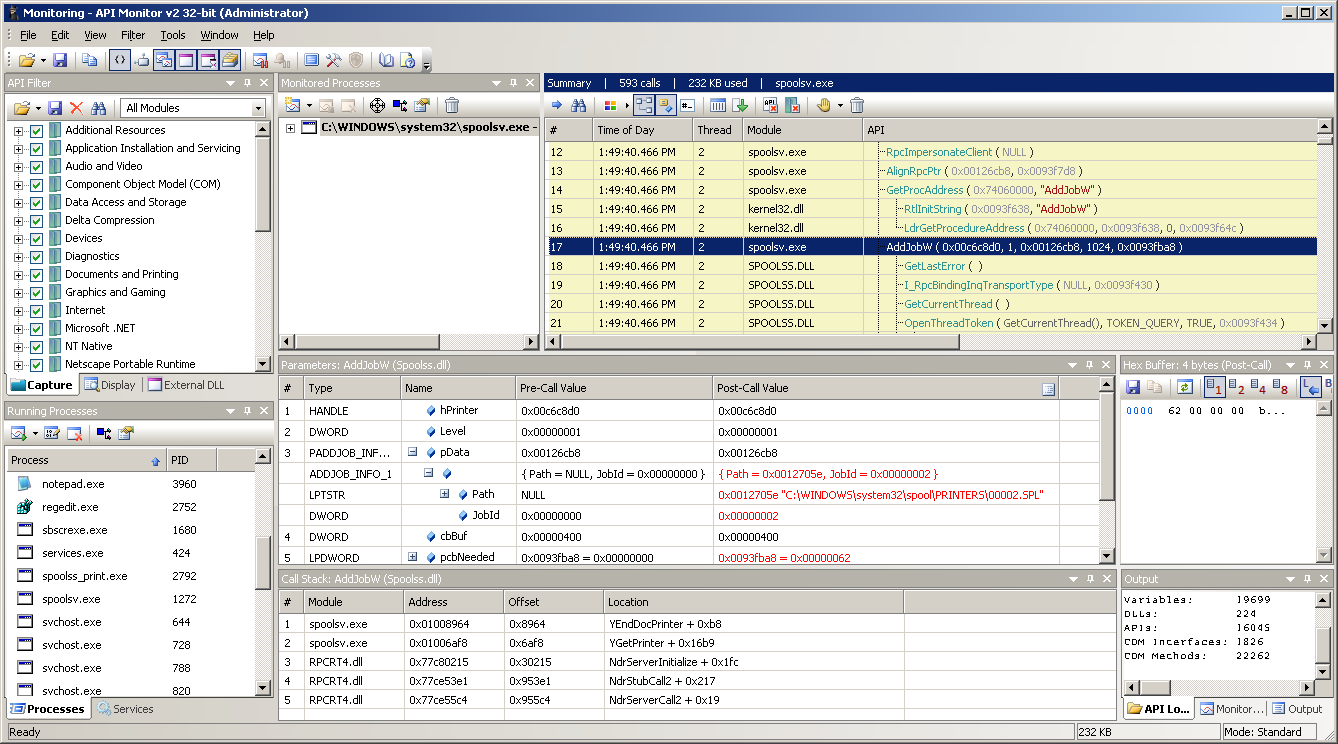
\includegraphics{images/apimon.png}
	\caption{Rohitab Batra's \glsdisp{API}{API} Monitor used to analyze an \glsdisp{RPC}{RPC} call to the Spooler Server in Windows Server 2003}
	\label{fig:APIMonitor}
\end{figure}


\subsection{WinDbg}
WinDbg is a debugger offered as a free download by Microsoft.
It supports debugging User-Mode and Kernel-Mode applications and is generally the debugger of choice for Windows driver developers due to its tight integration into the Microsoft development environment.
Kernel-Mode debugging can happen on the local system or on a remote computer that is connected through a Serial, FireWire, \gls{USB} or Ethernet cable.
In a next step, Windows is booted with the \gls{KD} Protocol enabled to let the debugger connect and afterwards break into every component of the operating system at any time.
This Protocol has also been adopted by the ReactOS Operating System to provide a debugging experience comparable to Windows.
That means, the same WinDbg application can be used to debug ReactOS just like a usual Windows environment.

WinDbg can retrieve information from \gls{PDB} files to provide single stepping through C/C++ source code files and detailed symbol information.
\gls{PDB} files are either generated by the Visual C++ compiler (for self-written applications) or downloaded from the Microsoft Symbol Server (for closed-source Windows components).
While latter ones do not reveal any source code of Windows components, the closed-source \gls{PDB} files make WinDbg aware of some variables and function names.
On top of this, WinDbg comes with a handful of extensions that provide several abstract views on the operating system state.
For example, this encompasses loaded processes and threads, bluescreen analysis, and hardware status information.
A typical WinDbg screen is shown in Figure~\ref{fig:WinDbg}.
With all these possibilities combined, WinDbg provides quite a powerful tool to gather information about any software under Windows or single step through it.


\begin{landscape}
	\begin{figure}
		\centering
		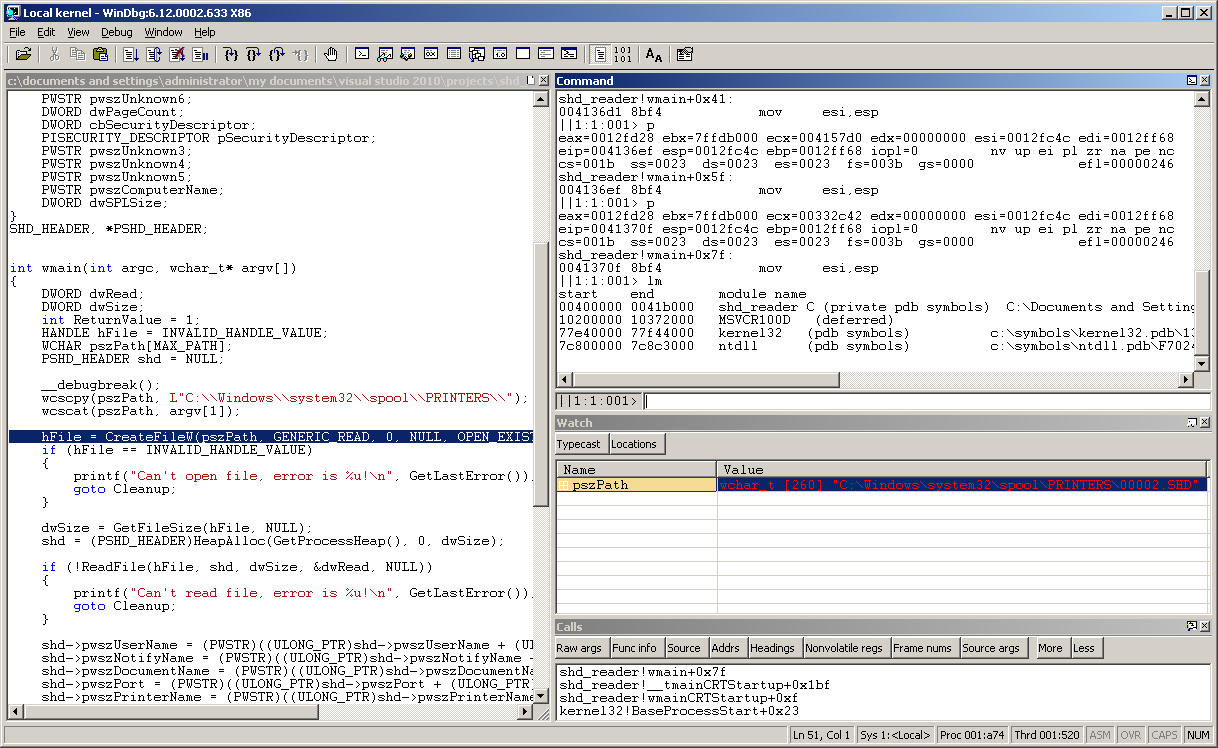
\includegraphics{images/windbg.png}
		\caption{WinDbg debugging a User-Mode application with loaded \glsdisp{PDB}{PDB} information in Windows Server 2003}
		\label{fig:WinDbg}
	\end{figure}
\end{landscape}
